% \section*{Final story line....}

% \begin{enumerate}
%     \item Introduction:
%         \begin{itemize}
%             \item Motivation:
%                 \begin{itemize}
%                     \item LPWAN is awesome and catching up
%                     \item Range and battery life problems (e.g. long battery life is conditional)
%                     \item LoRa networks are planned (UGWs are disorganized)
%                     \item Can we leverage UGWs to collate a decode weak signals?
%                     \item Should lead to improvement in client power and improvement in network range
%                 \end{itemize}
%             \item Why is it hard?
%                 \begin{itemize}
%                     \item is a SIMO/ joint decoding problem
%                         \begin{itemize}
%                             \item needs detection
%                             \item large amount of data transfer
%                         \end{itemize}
%                     \item Problems:
%                         \begin{itemize}
%                             \item Inefficient
%                             \item Not scalable
%                         \end{itemize}
%                     \item Need efficient local decoding scheme
%                     \item Need software architecture to enable this
%                         \begin{itemize}
%                             \item How to avoid wasted computations (e.g. through short circuit)
%                             \item Joint decoding
%                             \item Software architecture
%                             \item Result: improved scalability (due to shorter messaging times)
%                         \end{itemize}
%                 \end{itemize}
%             \item Contribution:
%                 \begin{itemize}
%                     \item Leveraging diversity with unplanned UGWs
%                     \item A hardware platform and underlying algorithms for IQ processing and local detection of LoRa preambles
%                     \item Software infrastructure for joint detection and improving scalability
%                 \end{itemize}
%         \end{itemize}
%     \item Related Work:
%         \begin{itemize}
%             \item LPWAN
%             \item SIMO (?) and diversity
%             \item Cloud-RAN (but our system has short and infrequent messages)
%         \end{itemize}
%     \item Background:
%         \begin{itemize}
%             \item SIMO Primer
%             \item LoRa
%             \item LoRaWAN
%         \end{itemize}
%     \item Architecture:
%         \begin{itemize}
%             \item The goal: decode weak transmission by collating information from multiple base-stations
%             \item Flow diagram (picture with cloudy and edgy stuff)
%             \item The strawman comparison: stream everything
%             \item Strawman limitations
%                 \begin{itemize}
%                     \item Weak signals and limited bandwidth (problems at gateways (could use joint decoding of preambles but cant afford to stream everything))
%                     \item Scaling issues (problems at the cloud)
%                 \end{itemize}
%         \end{itemize}
%     \item Gateway:
%         \begin{itemize}
%             \item Hardware + block diagram + capability + how to decode IQ streams
%             \item Local detection algorithm
%             \item Optional: (LoRa-aware) compression
%         \end{itemize}
%     \item Cloud:
%         \begin{itemize}
%             \item Q. How to solve scaling issues in the cloud?
%             \item Avoid wasted computations
%                 \begin{itemize}
%                     \item Short circuit
%                     \item Leverage locality of gateways (only use a subset of gateways for decoding)
%                 \end{itemize}
%             \item Spatial partitioning helps correctness and performance
%                 \begin{itemize}
%                     \item Leverage locality
%                     \item Leverage timing
%                 \end{itemize}
%             \item Shorter transmissions help scalability
%         \end{itemize}
%     \item Implementation
%      \begin{itemize}
%          \item OC Arch + additions over regular LoRaWAN
%          \item Drive and Penetration test results around campus for earlier deployment
%      \end{itemize}
%     \item Evaluation:
%         \begin{itemize}
%             \item Local packet detection: Error CDF vs SNR
%             \item Diversity gain: Usable spreading factors vs distance/SNR
%             \item Impact on client power: Device power trace, Battery life vs distance
%             \item Increased capacity due to sensitivity gain (in simulation)
%         \end{itemize}
%     \item Conclusions and Future Work:
%         \begin{itemize}
%             \item Extensions to MU-MIMO, tomography
%             \item Other stuff
%         \end{itemize}
% \end{enumerate}

\section{Introduction}
\label{sec:intro}

% Long distance high-quality communication systems are required to provide a large number of modern IoT services across sectors. 
Low Power Wide Area Networks (LP-WANs) are increasingly seen as an attractive
communication platform for city-scale Internet-of-Things (IoT) deployments.
They offer the ability to wirelessly connect energy-constrained devices to
gateways over distances of many kilometers. LP-WANs also have power and cost
advantages over alternatives like cellular networks, particularly in
deploy-once, low-maintenance and low throughput sensing applications.

While far from pervasive, the capabilities of LP-WANs like
LoRaWAN~\cite{Sornin2015, LoRaWanAlliance2015}, SigFox~\cite{centenaro2016}
and Ingenu's RPMA~\cite{Ingenu2015} have attracted investment and have spawned
early deployments. These technologies operate on unlicensed spectrum, allowing
businesses and consumers alike to deploy their own devices and gateways. With the
recent announcement by Comcast \cite{comcast, comcast2} to integrate LP-WAN
radios into future set-top boxes in the U.S., LP-WANs are likely to scale
rapidly. In fact, major cities in the U.S. are likely to see fast-paced LP-WAN
coverage, given that each LP-WAN gateway promises a range of up to ten
kilometers networking client devices powered by ten-year AA batteries~\cite{LoRaWanAlliance2015}.

%% Still have range and power issues
%% Swarun: Work in progress

Yet, despite the expected rapid rise in density of LP-WAN gateways, not all devices will experience the promised ten-year battery life. Specifically, devices located in urban spaces deep inside buildings or in remote neighborhoods will experience severe drain in battery as their signals are highly attenuated even at the closest base station. Some of these devices -- such as those in basements or tunnels -- may not be in communication range of any gateway at all. Unlike cellular networks, LP-WANs are largely user deployed and unplanned, meaning that these devices may remain battery-deprived or simply out of network reach in perpetuity, even as thousands of gateways continue to spring up city-wide.  



This paper presents \name, a system that enhances the battery-life and
coverage of LP-WAN clients in large urban deployments. \name\ exploits the
observation that while signals from certain clients may attenuate significantly, they are still likely to be received by multiple gateways in a dense network. \name\ develops a hardware and software design at the gateways that identifies and transports weak received signals to the cloud. We then develop a joint decoding system at the cloud that coherently
combines weak signals received across multiple city gateways to decode the underlying data. As a result, \name\ both expands the decoding range of the LP-WAN network and improves battery-life for nodes already in range -- allowing clients across the network to spend less energy per transmitted bit. We implement \name\ on the LoRaWAN platform~\cite{LoRaWanAlliance2015}, a popular and widely available LP-WAN technology. \name\ is
implemented in a first-of-its-kind low-power wide-area pilot deployment for
coherent diversity combining. This deployment serves a large neighborhood of a major U.S. city and
demonstrates increased coverage and battery-life across clients in the network.

% % Intro to LoRa and LoRaWAN that introduces all the necessary terminology

% % Swarun: I am dropping this.. too much background for the intro.. I want to know about Charm now!
% LoRa is an emerging LP-WAN technology from Semtech that uses chirp
% spread-spectrum that trades off low bit rate for long range. An important
% parameter is the spreading factor: different spreading factors can be
% independently received and end up affecting the transmission time, bit rate
% and sensitivity of the transmission. LoRaWAN defines the higher levels of the
% networking stack that enable device-centric unidirectional or bi-directional
% communication. LoRaWAN gateways are typically inexpensive, simple forwarders
% that send all decoded packets to a server in the cloud over a regular internet
% connection, the cloud-server then decides which gateways should respond.
% LoRaWAN also allows and encourages clients to deploy their own unplanned
% gateways (which we call \textit{user-deployed gateway} or \textit{UGW}) to
% expand the coverage of the network.

\begin{figure}
    \centering
    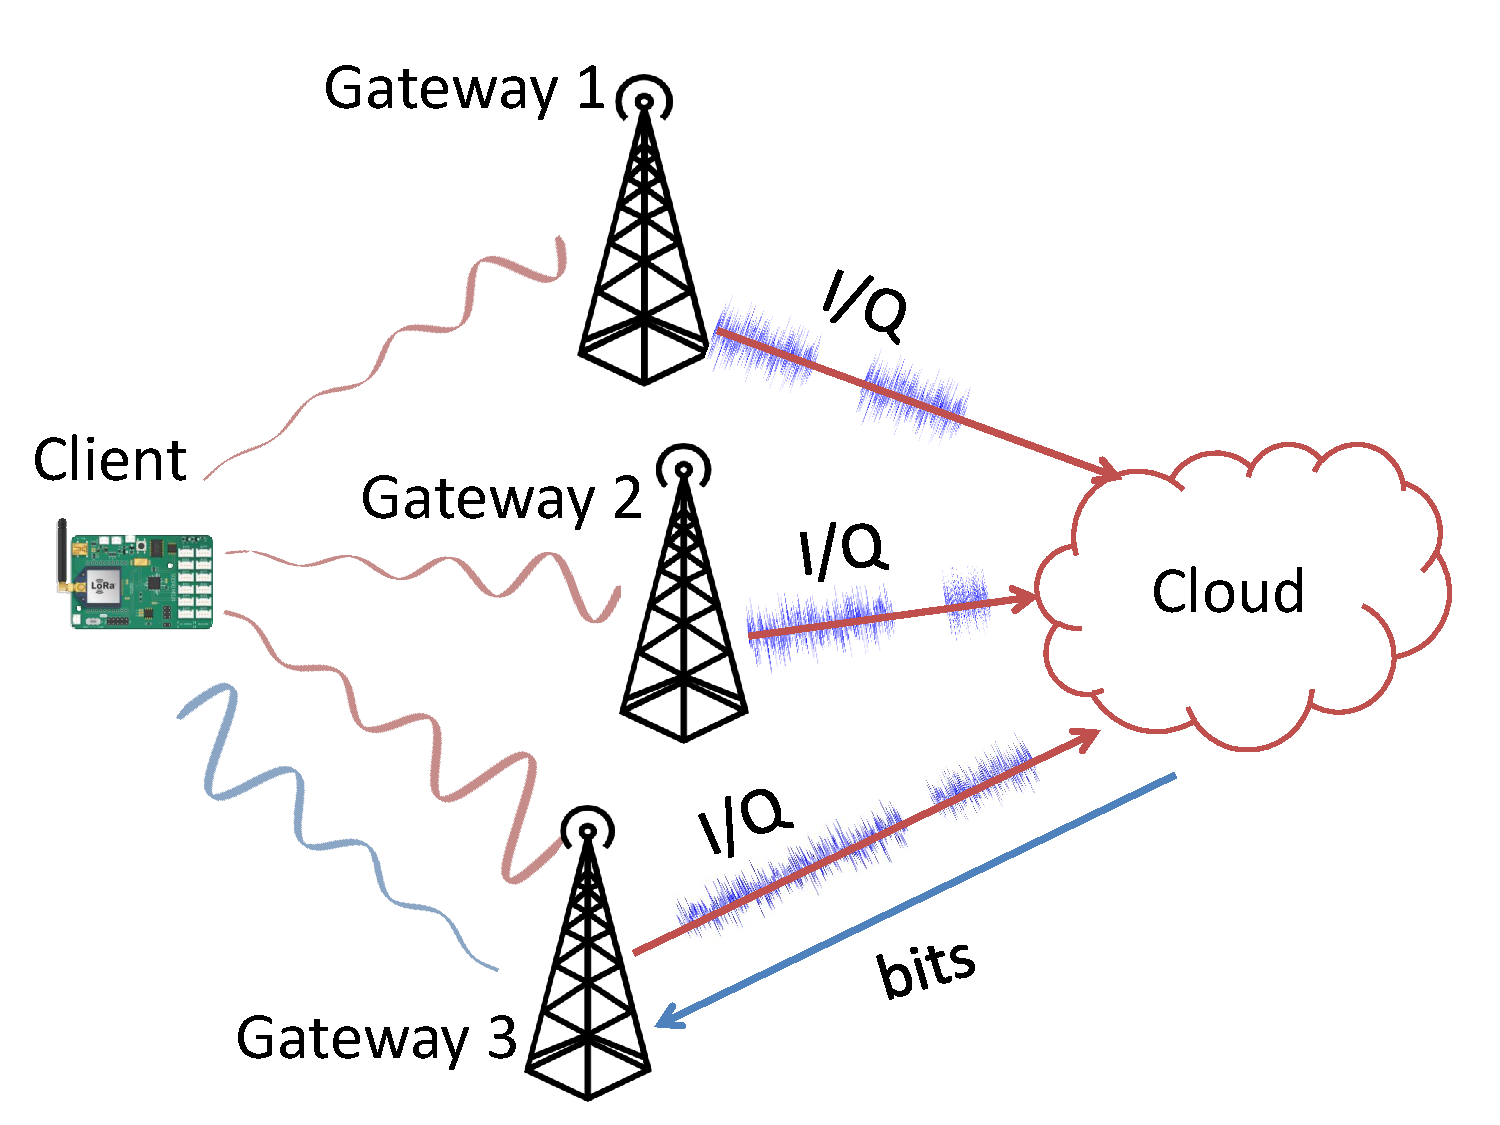
\includegraphics[width=0.30\textwidth]{location-aware-network/figures/LoRaRAN.pdf}
        \vspace*{-0.1in}
    \caption{Charm: LP-WAN joint decoding in the cloud}
    \vspace*{-0.1in}
    \label{fig:my_label}
    \compactimg
\end{figure}

% {\color{blue} (Intuitively, explain how does Charm's approach actually leads
% to client power savings)} 

% % Swarun: Dont lie range argument
% Charm allows users who are in range to transmit at
% faster data rates that would not have been decodable using a single gateway
% receiver. This allows for more air time for weaker transmissions from further
% away clients.

% Why is it hard?

While coherent diversity combining and PHY-layer processing in the cloud has received much attention in the Wi-Fi~\cite{tan2009sam, xie2014scalable} and cellular~\cite{checko2015cloud, wubben2014benefits} context, designing such a system for low-power WANs offers radically new challenges. At the gateways,  LP-WAN signals are often too weak to be ordinarily detected -- more than 30 dB below the noise floor. Yet, simply shipping all received data to the cloud would overwhelm the backend link, which is often  a simple home LAN. At the cloud, collating receptions from a large number of gateways at city-scale to identify which of them contain packets from the same user is a challenge. We provide an overview of our approach to address each of these challenges below. 

% Yet, designing a system that can coherently combine weak signals across LP-WAN gateways at the cloud is challenging for several reasons. At the gateways, 
% The main challenges in designing a city-scale joint-decoding system stem from
% three main causes: 1. very weak receptions, 2. limited bandwidth from the
% gateway to the cloud server and 3. challenges in scaling at the cloud.

\textbf{Noise-Resilience at the Gateway:} The key challenge at the gateway is identifying packets that are significantly below the noise and therefore virtually undetectable. A strawman approach to this problem would be to correlate the received signal with a known preamble in any valid packet. For instance, LoRaWAN uses a sequence of identical chirps -- signals whose frequency increases linearly in time -- as a signature prefixing every packet. In principle, sending an extremely long preamble could provide high resilience to noise. In practice, doing so goes against the spirit of LP-WANs where energy for transmission at the clients is a valuable resource. 

\name's approach to resolve this challenge is a hardware and software gateway design that leverages the structure of the LoRaWAN LP-WAN protocol. Specifically, we develop a transform that converts the data symbols containing \textit{a priori} unknown bits into a repeated and known sequence of signals much like the preamble. \name\ can therefore now use both the preamble and the modified data sequence to detect any packet. 


To understand our approach at a high-level, we present an illustrative example that dives into the details of the LoRaWAN PHY-layer. Specifically, LoRaWAN transmits data symbols as chirps whose initial frequency is a function of the data. For instance over a bandwidth of 100 Hz, LoRa could represent the bit "0" as a chirp starting at 2 Hz and bit "1" as a chirp starting at 52 Hz. \name's filter aliases the received LoRa signal so that frequencies modulo 50 Hz fold into each other. This means that both bit "0" and bit "1" now map to an identical chirp starting at 2 Hz. We therefore apply this filter through the received packet to obtain a repeated sequence of chirps as long as the entire packet itself. This allows us to detect the packet with a much higher resilience to noise compared to using the preamble alone, without incurring additional overhead. 

We develop a custom gateway hardware platform integrating a SemTech LoRaWAN radio frontend, a low-power FPGA and Raspberry PI that can filter and detect weak signals by processing received raw I/Q samples in real-time. Our hardware platform is designed to be open and highly programmable -- a novel tool to experiment with alternative LP-WAN PHY-layer designs in the 900 MHz ISM band, without compromising on signal quality or real-time performance. 
 


% Gateways receive transmissions from
% distant clients which are far below the noise floor. These transmissions are
% not only difficult to detect but also cannot be decoded independently.
% {\color{blue} (Add actual numbers?)} Using an approach similar to
% {\color{red}~\cite{} (Cloud RAN?)} would require continuously streaming all
% the raw received signals to a cloud-based decoder for both detection and
% decoding. Such an approach places a heavy cost on the internet bandwidth
% between the gateway and the cloud, which is particularly infeasible for UGWs.% This means the devices will have to continuously stream all their received raw signal data through a backbone for packet detection and decoding the data. 
% This imposes a huge cost on the bandwidth of the backbone and also is also infeasible at low latency.
% To make matters worse, the received signals are challenging to synchronize, given the timing and frequency offsets between the base stations themselves. 

% Although LoRaWAN gateways are very capable, they do not provide the raw
% baseband quadrature signals which are required for joint decoding. We
% developed a low-cost auxiliary platform, called LPRAN that uses a similar
% radio frontend combined with a FPGA and Raspberry Pi for local signal
% processing. This auxiliary hardware behaves like a software-defined radio in
% the 900 MHz ISM band, generating processed quadrature streams and computing
% local parameters (like spreading factor and center frequency which are
% necessary inputs for the cloud-decoding algorithm).

% Our solution to the bandwidth limitation problem leverages the structure of
% LoRaWAN LP-WAN packets. We develop a solution that detects LoRaWAN packets
% even if they are 37~dB below the noise floor and therefore remain completely
% non-decodable. Our solution exploits the presence of a large number of
% repeated preambles in LoRaWAN (up to 16 in the standard). Specifically, we
% correlate the received sequence with long-sequences of LoRaWAN chirps to
% detect the locations of packets. We repeat this process across gateways and
% quickly alert neighboring base stations, should a preamble be detected. The
% base station also does this for correctly decoded packets -- eliminating the
% need for base stations to upload weak signals for packets already decoded.
% Owing to the lenient latency constraints for acknowledgement of a packet in
% LoRaWAN (one to two seconds), our approach readily scales to a large-scale
% network. In effect, our approach therefore only streams to the cloud signals
% that correspond to valid packets.

\noindent \textbf{Scalability at the Cloud:} At the cloud, \name\ must deal with a large number of receptions from various gateways in a city, pruning for weak signals and identifying common signals between gateways. \name\ proposes multiple optimizations to run its algorithms seamlessly at city-scale. For instance, it is often the case that gateways transmit weak signals to the cloud for packets that have already been decoded perfectly at other gateways. Yet, realizing that the weak signal has already been decoded elsewhere is impossible without decoding it in the cloud in the first place. \name\ resolves this chicken-or-egg dilemma by exploiting both the timing and geographical location of the received signal. Prior to sending any signal data to the cloud, a \name\ gateway sends the location, accurate timing and signal-to-noise ratio of the received weak packet. The cloud collates such information across multiple gateways and requests for signals only from the gateways that receive these signals the best. In doing so, \name\ saves valuable uplink bandwidth at the gateways and compute cycles at the cloud. We describe how \name\ mitigates  range of other important challenges at the cloud such as imperfect timing, frequency offsets and overlapping transmissions. 



% {\color{blue} (This section still needs
% lots of work)} Another challenge Charm must deal with given its expanded
% coverage, is the problem of processing a large number of streams to be
% combined and decoded.

% {\color{blue} Points to cover:
% \begin{itemize}
%     \item How to avoid wasted computations through our distributed algorithm
%     (short-circuiting, selectively combining streams based on location,
%     frequency and time)
%     \item How is this scalable? i.e. why can we support more nodes in the
%     network now? (transmit time decreases)
%     \item What is the software/cloud infrastructure required to support these
%     operations?
% \end{itemize}
%}
% Indeed, one would imagine that given that Charm serves a much larger coverage area, it scales poorly owing to collisions between users already in the network and users who newly gain coverage. 
% Counter-intuitively, we observe that in practice this is not the case. 

% We show how Charm scales despite collisions from transmissions in different geographical neighborhoods by exploiting spatial reuse -- the fact that some base stations are closer to one neighborhood and farther than the other. {\color{blue} Mention things like short-circuiting. }

%Coherent combination of packets requires inversion of individual channel effects on each of the data stream. However, across a packet the effects of the channel can be estimated by extrapolation of the channel effects at the preamble. This means we can estimate the channel at the preamble(which we can compare with a standard preamble to get the channel) and expect it to follow the same hardware offset drift pattern across the rest of the packet. Using this channel measurement we can invert the effect of channel and get all the signals in phase which we can then constructively combine to receive the packet at a much higher SNR.

We evaluate \name\ on a large university campus with four rooftop gateways and eight indoor user-deployed gateways built using our custom hardware platform. We study \name's coverage and performance indoors and outdoors  across a 10 square kilometer area surrounding the campus. Our results reveal the following:

%{\color{blue} (Add some introduction about the nature of experiments.)} In our evaluations, we demonstrate the following:
\begin{itemize}
    \item {\bf Battery-Life: }\name\ improves the signal to noise ratio at a typical LoRaWAN client by coherently combining across 8 base stations by 3.16 dB, extending battery life by a factor of 4.
    \item {\bf Range: } We improve the maximum communication range of 8 indoor user-deployed gateways in urban settings from 60m in LoRaWAN to 200 meters using \name, an overall increase of 10x coverage area 
    \item {\bf Coverage: } Our trace-driven simulation based on city-wide drive tests, estimates an overall increase in coverage by up to a factor of 2 due to \name\ over LoRaWAN. 
\end{itemize}

ok1
\textbf{Contributions:} We make the following novel contributions:
\begin{itemize}
    \item A technique that leverages the geographical diversity of unplanned user-deployed gateways to enable joint decoding of weak transmissions. This improves battery-life for users in the network and increases the coverage area.
    \item A hardware platform and the underlying algorithms for detecting weak LoRaWAN transmissions locally. 
    \item A software architecture that builds atop of LoRaWAN to enable joint-decoding of signals in a scalable manner.
\end{itemize}

















% % \section*{Final story line....}

% % \begin{enumerate}
% %     \item Introduction:
% %         \begin{itemize}
% %             \item Motivation:
% %                 \begin{itemize}
% %                     \item LPWAN is awesome and catching up
% %                     \item Range and battery life problems (e.g. long battery life is conditional)
% %                     \item LoRa networks are planned (UGWs are disorganized)
% %                     \item Can we leverage UGWs to collate a decode weak signals?
% %                     \item Should lead to improvement in client power and improvement in network range
% %                 \end{itemize}
% %             \item Why is it hard?
% %                 \begin{itemize}
% %                     \item is a SIMO/ joint decoding problem
% %                         \begin{itemize}
% %                             \item needs detection
% %                             \item large amount of data transfer
% %                         \end{itemize}
% %                     \item Problems:
% %                         \begin{itemize}
% %                             \item Inefficient
% %                             \item Not scalable
% %                         \end{itemize}
% %                     \item Need efficient local decoding scheme
% %                     \item Need software architecture to enable this
% %                         \begin{itemize}
% %                             \item How to avoid wasted computations (e.g. through short circuit)
% %                             \item Joint decoding
% %                             \item Software architecture
% %                             \item Result: improved scalability (due to shorter messaging times)
% %                         \end{itemize}
% %                 \end{itemize}
% %             \item Contribution:
% %                 \begin{itemize}
% %                     \item Leveraging diversity with unplanned UGWs
% %                     \item A hardware platform and underlying algorithms for IQ processing and local detection of LoRa preambles
% %                     \item Software infrastructure for joint detection and improving scalability
% %                 \end{itemize}
% %         \end{itemize}
% %     \item Related Work:
% %         \begin{itemize}
% %             \item LPWAN
% %             \item SIMO (?) and diversity
% %             \item Cloud-RAN (but our system has short and infrequent messages)
% %         \end{itemize}
% %     \item Background:
% %         \begin{itemize}
% %             \item SIMO Primer
% %             \item LoRa
% %             \item LoRaWAN
% %         \end{itemize}
% %     \item Architecture:
% %         \begin{itemize}
% %             \item The goal: decode weak transmission by collating information from multiple base-stations
% %             \item Flow diagram (picture with cloudy and edgy stuff)
% %             \item The strawman comparison: stream everything
% %             \item Strawman limitations
% %                 \begin{itemize}
% %                     \item Weak signals and limited bandwidth (problems at gateways (could use joint decoding of preambles but cant afford to stream everything))
% %                     \item Scaling issues (problems at the cloud)
% %                 \end{itemize}
% %         \end{itemize}
% %     \item Gateway:
% %         \begin{itemize}
% %             \item Hardware + block diagram + capability + how to decode IQ streams
% %             \item Local detection algorithm
% %             \item Optional: (LoRa-aware) compression
% %         \end{itemize}
% %     \item Cloud:
% %         \begin{itemize}
% %             \item Q. How to solve scaling issues in the cloud?
% %             \item Avoid wasted computations
% %                 \begin{itemize}
% %                     \item Short circuit
% %                     \item Leverage locality of gateways (only use a subset of gateways for decoding)
% %                 \end{itemize}
% %             \item Spatial partitioning helps correctness and performance
% %                 \begin{itemize}
% %                     \item Leverage locality
% %                     \item Leverage timing
% %                 \end{itemize}
% %             \item Shorter transmissions help scalability
% %         \end{itemize}
% %     \item Implementation
% %      \begin{itemize}
% %          \item OC Arch + additions over regular LoRaWAN
% %          \item Drive and Penetration test results around campus for earlier deployment
% %      \end{itemize}
% %     \item Evaluation:
% %         \begin{itemize}
% %             \item Local packet detection: Error CDF vs SNR
% %             \item Diversity gain: Usable spreading factors vs distance/SNR
% %             \item Impact on client power: Device power trace, Battery life vs distance
% %             \item Increased capacity due to sensitivity gain (in simulation)
% %         \end{itemize}
% %     \item Conclusions and Future Work:
% %         \begin{itemize}
% %             \item Extensions to MU-MIMO, tomography
% %             \item Other stuff
% %         \end{itemize}
% % \end{enumerate}

% \section{Introduction}
% \label{sec:intro}

% % Long distance high-quality communication systems are required to provide a large number of modern IoT services across sectors. 
% Low Power Wide Area Networks (LP-WANs) are increasingly seen as an attractive
% communication platform for city-scale Internet-of-Things (IoT) deployments.
% They offer the ability to wirelessly connect energy-constrained devices to
% gateways over distances of many kilometers. LP-WANs also have power and cost
% advantages over alternatives like cellular networks, particularly in
% deploy-once, low-maintenance and low throughput sensing applications

% While far from pervasive, the capabilities of LP-WANs like
% LoRaWAN~\cite{Sornin2015, LoRaWanAlliance2015}, SigFox~\cite{centenaro2016}
% and Ingenu's RPMA~\cite{Ingenu2015} have attracted investment and have spawned
% early deployments. These technologies operate on unlicensed spectrum, allowing
% businesses and consumers alike to deploy their own base stations. With the
% recent announcement by Comcast {\color{red}~\cite{}} to integrate LP-WAN
% radios into future set-top boxes in the U.S., LP-WANs are likely to scale
% rapidly. Indeed, major cities in the U.S. are likely to see fast-paced LP-WAN
% coverage, given that each LP-WAN base station promises a range of up to ten
% kilometers~\cite{LoRaWanAlliance2015}.

% %% Still have range and power issues
% %% TODO: elaborate exactly what these issues are
% Yet, the maximum range of LP-WAN base stations of ten kilometers comes at a
% cost -- battery-drain. Specifically, the further an LP-WAN device is from a
% base station, the more power it is likely to expend to transmit the same
% amount of information{\color{red}~\cite{}}. {\color{blue} (Sudden jump from
% LP-WAN to LoRaWAN... What is the knob that enables jumping from 1 year to 10
% years?)} In practical terms for instance, this reduces the battery life of a
% LoRaWAN device from 10-years when in close proximity of the base station to
% just 2 years at maximum range{\color{red}~\cite{}}. {\color{blue} (The suburban
% argument is not convincing (and may not even be true). Focus on battery and
% more uniform coverage.)} Given that LP-WANs base station deployments will be
% at their densest in cities, suburban areas are likely to bear the brunt of
% poor performance and reduced battery life. {\color{blue} (Add some actual
% power numbers.)} More fundamentally, LP-WANs unlike cellular deployments are
% unlicensed and unplanned, meaning that the outermost suburban neighborhoods
% may simply be beyond the range of LP-WAN coverage, while cities remain
% over-provisioned.


% This paper presents Charm, a system that enhances the battery-life and
% coverage of LoRaWAN clients in large urban deployments. Charm exploits the
% observation that while signals from a distant and hard to reach clients may
% attenuate significantly, they are still likely to be received by multiple base
% stations. Charm develop a collaborative joint-decoding system that coherently
% combines weak signals heard across multiple city base stations to decode the
% underlying information. As a result, it both expands the decoding range of the
% LP-WAN network and improves battery-life for nodes already in range. Charm is
% implemented in a first-of-its-kind low-power wide-area pilot deployment of
% joint decoding serving a large neighborhood of a major U.S. city and
% demonstrates increased coverage and battery-life for nodes in surrounding
% neighborhoods.

% % Intro to LoRa and LoRaWAN that introduces all the necessary terminology
% LoRa is an emerging LP-WAN technology from Semtech that uses chirp
% spread-spectrum that trades off low bit rate for long range. An important
% parameter is the spreading factor: different spreading factors can be
% independently received and end up affecting the transmission time, bit rate
% and sensitivity of the transmission. LoRaWAN defines the higher levels of the
% networking stack that enable device-centric unidirectional or bi-directional
% communication. LoRaWAN gateways are typically inexpensive, simple forwarders
% that send all decoded packets to a server in the cloud over a regular internet
% connection, the cloud-server then decides which gateways should respond.
% LoRaWAN also allows and encourages clients to deploy their own unplanned
% gateways (which we call \textit{user-deployed gateway} or \textit{UGW}) to
% expand the coverage of the network.

% \begin{figure}
%     \centering
%     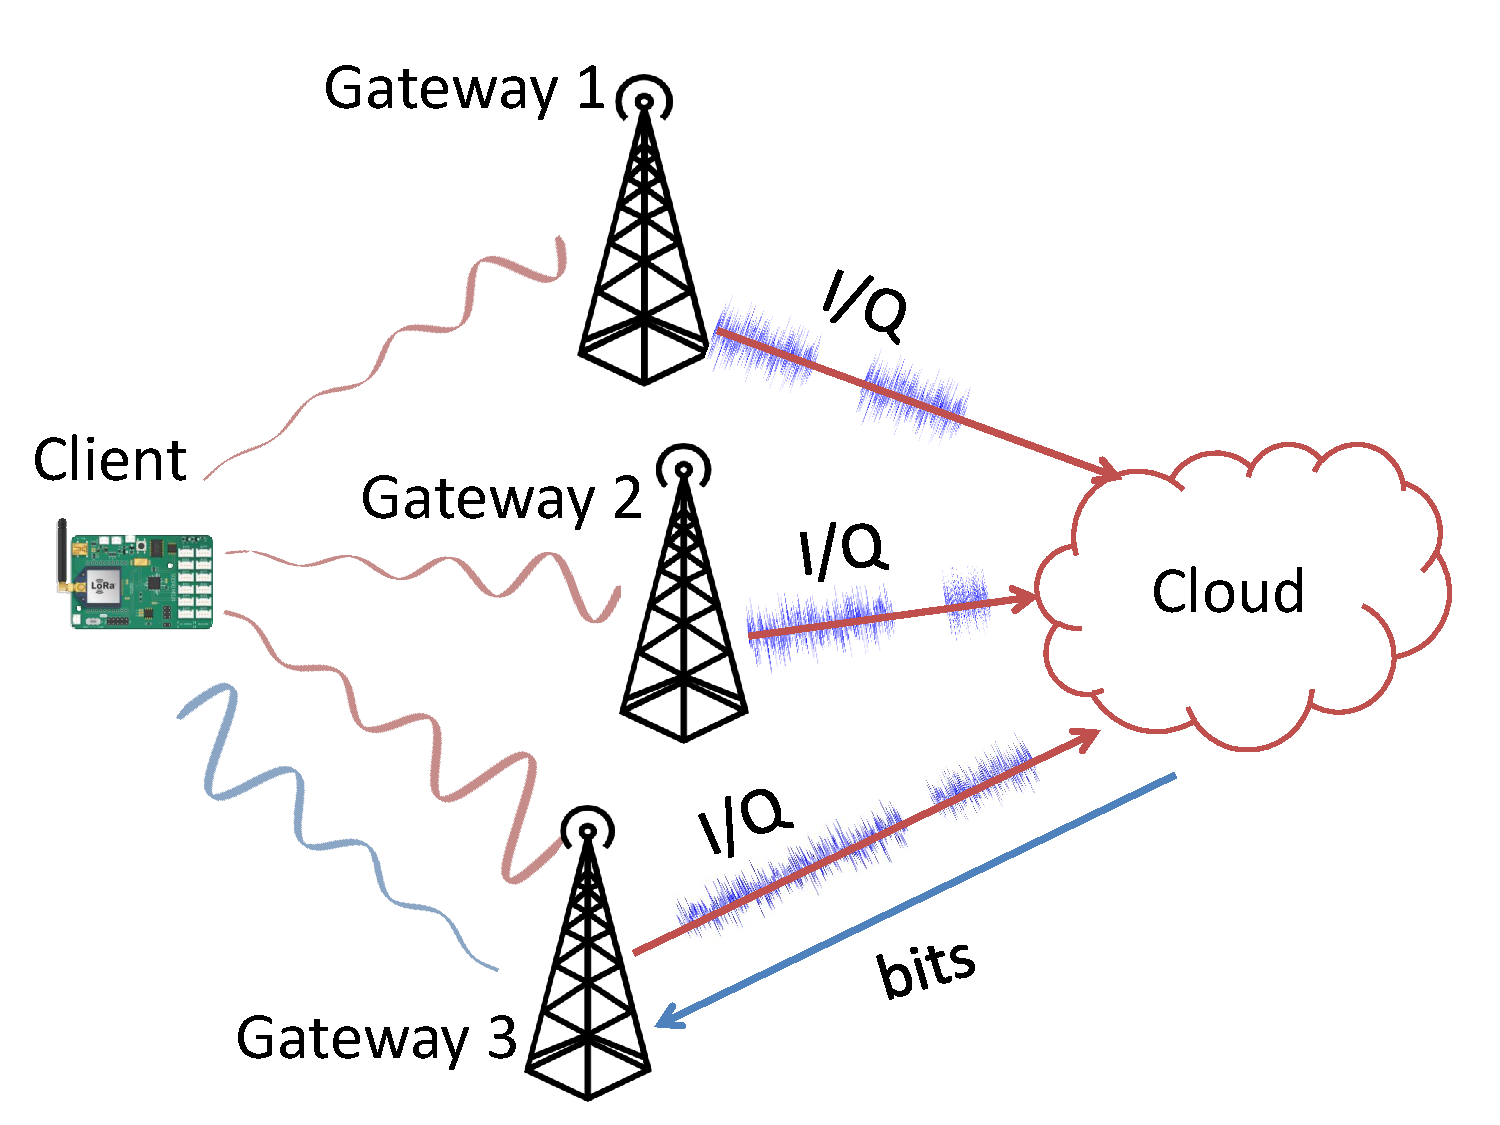
\includegraphics[width=0.45\textwidth]{location-aware-network/figures/LoRaRAN.pdf}
%     \caption{Charm:Distributed LPWAN communication system}
%     \label{fig:my_label}
% \end{figure}

% {\color{blue} (Intuitively, explain how does Charm's approach actually leads
% to client power savings)} Charm allows users who are in range to transmit at
% faster data rates that would not have been decodable using a single gateway
% receiver. This allows for more air time for weaker transmissions from further
% away clients.

% % Why is it hard?
% The main challenges in designing a city-scale joint-decoding system stem from
% three main causes: 1. very weak receptions, 2. limited bandwidth from the
% gateway to the cloud server and 3. challenges in scaling at the cloud.

% \textit{Challenges at the Gateway:} Gateways receive transmissions from
% distant clients which are far below the noise floor. These transmissions are
% not only difficult to detect but also cannot be decoded independently.
% {\color{blue} (Add actual numbers?)} Using an approach similar to
% {\color{red}~\cite{} (Cloud RAN?)} would require continuously streaming all
% the raw received signals to a cloud-based decoder for both detection and
% decoding. Such an approach places a heavy cost on the internet bandwidth
% between the gateway and the cloud, which is particularly infeasible for UGWs.% This means the devices will have to continuously stream all their received raw signal data through a backbone for packet detection and decoding the data. 
% % This imposes a huge cost on the bandwidth of the backbone and also is also infeasible at low latency.
% % To make matters worse, the received signals are challenging to synchronize, given the timing and frequency offsets between the base stations themselves. 

% Although LoRaWAN gateways are very capable, they do not provide the raw
% baseband quadrature signals which are required for joint decoding. We
% developed a low-cost auxiliary platform, called RFTAP that uses a similar
% radio frontend combined with a FPGA and Raspberry Pi for local signal
% processing. This auxiliary hardware behaves like a software-defined radio in
% the 900 MHz ISM band, generating processed quadrature streams and computing
% local parameters (like spreading factor and center frequency which are
% necessary inputs for the cloud-decoding algorithm).

% Our solution to the bandwidth limitation problem leverages the structure of
% LoRaWAN LP-WAN packets. We develop a solution that detects LoRaWAN packets
% even if they are 37~dB below the noise floor and therefore remain completely
% non-decodable. Our solution exploits the presence of a large number of
% repeated preambles in LoRaWAN (up to 16 in the standard). Specifically, we
% correlate the received sequence with long-sequences of LoRaWAN chirps to
% detect the locations of packets. We repeat this process across gateways and
% quickly alert neighboring base stations, should a preamble be detected. The
% base station also does this for correctly decoded packets -- eliminating the
% need for base stations to upload weak signals for packets already decoded.
% Owing to the lenient latency constraints for acknowledgement of a packet in
% LoRaWAN (one to two seconds), our approach readily scales to a large-scale
% network. In effect, our approach therefore only streams to the cloud signals
% that correspond to valid packets.

% \textit{Scalability at the Cloud:} {\color{blue} (This section still needs
% lots of work)} Another challenge Charm must deal with given its expanded
% coverage, is the problem of processing a large number of streams to be
% combined and decoded.

% {\color{blue} Points to cover:
% \begin{itemize}
%     \item How to avoid wasted computations through our distributed algorithm
%     (short-circuiting, selectively combining streams based on location,
%     frequency and time)
%     \item How is this scalable? i.e. why can we support more nodes in the
%     network now? (transmit time decreases)
%     \item What is the software/cloud infrastructure required to support these
%     operations?
% \end{itemize}
% }
% % Indeed, one would imagine that given that Charm serves a much larger coverage area, it scales poorly owing to collisions between users already in the network and users who newly gain coverage. 
% % Counter-intuitively, we observe that in practice this is not the case. 

% % We show how Charm scales despite collisions from transmissions in different geographical neighborhoods by exploiting spatial reuse -- the fact that some base stations are closer to one neighborhood and farther than the other. {\color{blue} Mention things like short-circuiting. }

% %Coherent combination of packets requires inversion of individual channel effects on each of the data stream. However, across a packet the effects of the channel can be estimated by extrapolation of the channel effects at the preamble. This means we can estimate the channel at the preamble(which we can compare with a standard preamble to get the channel) and expect it to follow the same hardware offset drift pattern across the rest of the packet. Using this channel measurement we can invert the effect of channel and get all the signals in phase which we can then constructively combine to receive the packet at a much higher SNR.

% {\color{blue} (Add some introduction about the nature of experiments.)} In our evaluations, we demonstrate the following:
% \begin{itemize}
%     \item We improve the range at SF 7 by XXX m, SF 10 by YYY m , and SF 12 by
%     ZZZ m.
%     \item With 8 base stations, we can add X m$^2$ more area to our coverage area.
%     \item We can achieve gains of J dBW,K dBW and LdBW for the signal using 3,
%     6 and 8 base stations, respectively.
%     \item We require overheads of K MBps and provide a latency of T ms for
%     detection and decoding of a packet with 8 base stations.
% \end{itemize}


% \textbf{Contributions:} In this paper we present the following novel contributions.
% \begin{itemize}
%     \item A technique that leverages the geographical diversity of unplanned
%     user-deployed gateways to enable joint decoding of weak transmissions.
%     This improves the quality-of-service for under-privileged users and increases the coverage area.
%     \item A hardware platform and the underlying algorithms for processing
%     quadrature streams and detection of LoRa preambles in weak transmissions,
%     both done locally. To reduce gateway internet bandwidth requirements, we
%     also introduce a scheme that selectively forwards a subset of probable
%     candidates to a cloud-based joint decoder.
%     \item A software architecture that builds on top of LoRaWAN to enable
%     joint-decoding of transmissions in a scaleable manner.
% \end{itemize}